\section{Recherche de solution}

\subsection{L'algorithme de Canny}
La première solution que nous testons est le filtre de Canny. Nous avons pu voir ce filtre durant
nos cours et nous trouvons que c'est une piste intéressante, car cette algorithme détecte les contours
présents dans une image.

\subsubsection{Version de base}
Le filtre de Canny a été créé en 1986 dans le but d'améliorer les résultats du filtre de Sobel.
Le principe du filtre est d'utiliser deux seuils, un seuil haut et un seuil bas. L'algorithme
commence par sélectionner les pixels supérieurs au seuil haut, puis recherche à partir de chaque
pixel en dessous du seuil haut les pixels qui sont au-dessus du seuil bas dans son voisinage. 
Chaque voisin qui est entre les deux seuils appartient à un contour, on passe donc sa valeur à
255 pour le prendre en compte dans celui-ci.\\ 
%Ainsi on voit que cet algorithme prend en compte deux caractéristiques, l'intensité et la direction du
%gradient de l'image.\\

Nous utilisons cet algorithme dans les régions autour des yeux afin de délimiter le contour
de chaque oeil. Nous testons cette algorithme avec différent seuil afin de voir si celui-ci
peut être intéressant dans notre situation. On voit sur les résultat que si le seuil est trop
bas l'oeil n'est pas détecter, et si le seuil est trop haut les rides de la personne dans la vidéo
apparaissent. Afin d'avoir un seuil adaptatif, nous prenons la valeur moyenne des pixels de l'image, ce
qui nous donne un résultat où le sourcil apparait et ou une partie de l'oeil est détecté.

%Le résultat permet de faire ressortir l'oeil, mais aussi les sourcils et certaines
%ombres présentent dans le creux de l'oeil. Ce filtre permet donc de détecter les contours des yeux,
%mais le résultat comporte soit beaucoup de bruit, soit trop peu de détails. Dans un premier
%temps, pour obtenir un seuil adaptatif, nous prenons la moyenne des pixels.

\begin{figure}[H]
 \center
 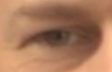
\includegraphics[width=4cm]{image/original.png}
 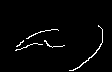
\includegraphics[width=4cm]{image/canny_moyenne.png}
 \caption{Image de test et résultat de l'algorithme de Canny avec une moyenne des pixels}
\end{figure}

On voit que cette méthode, n'est pas optimale et supprime trop d'informations. De plus,
l'algorithme prend en compte les ombres présentes dans l'image. Nous devons adapté cette méthode
afin de mieux détecter les contours dans les zones que nous souhaitons.

\subsubsection{Avec une moyenne de pixels sur des parties d'image}

Plutôt, que de prendre la moyenne des pixels sur l'ensemble de l'image de la zone péri-oculaire, nous segmentons l'image
en plusieurs zones dans lesquels nous calculons la moyenne et où nous effectuons l'algorithme
de Canny.

\begin{figure}[H]
 \center
 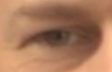
\includegraphics[width=4cm]{image/original.png}
 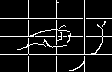
\includegraphics[width=4cm]{image/canny_decomposition.png}
 \caption{Image de test et résultat de l'algorithme de Canny avec division de l'image en 16}
\end{figure}

Avec cette méthode, nous obtenons une image bruité avec les bords de chaque rectangle utilisés
pour le calcul précédent, car l'algorithme de Canny ne prend pas en compte les bords de l'image
qu'il traite. Avec ce bruit nous ne pouvons clairement pas effectuer une recherche de l'oeil dans
l'image. Il nous faut donc trouver une solution pour supprimer les traits présents dans l'image
sans supprimer les contours présents dans l'image résultante.

\subsection{Ouverture des sous-images}

La dilatation d'une image est une opération morphologique\footnote{filtre non linéaire} qui utilise 
un élément structurant afin d'effectuer une convolution de l'image. Si l'un des voisins du pixel traité
est blanc alors celui-ci sera blanc, sinon il sera noir.
Cette opération a, en général, pour effet d'élargir une forme et de combler les trous qui peuvent être présent
dans cette forme. Nous avons également l'opération inverse qui est l'érosion, qui va diminuer la surface de la forme.
Lorsqu'une dilatation est effectuée sur une image en niveau de gris, le pixel traité prend la valeur maximum parmi
ses voisins, et le minimum pour la dilatation.\\

L'ouverture est la combinaison des deux opérations morphologiques vues précédemment, en commençant par 
l'érosion puis la dilatation. Cela a pour effet de fusionner des formes si elles sont proches (dans ce
cas il y a des chances que ce soit la même forme) et de diminuer la largeur de la forme pour 
s'approcher de la forme réel.\\ 

Afin de supprimer le bruit présent dans l'image de l'oeil après utilisation du filtre de Canny, nous effectuons une ouverture
de chaque sous image.

\begin{figure}[H]
 \center
 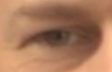
\includegraphics[width=4cm]{image/original.png}
 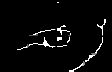
\includegraphics[width=4cm]{image/canny_final.png}
 \caption{Image de test et résultat de l'algorithme de Canny avec dilatation puis érosion des sous-images}
\end{figure}

Grâce à ce procédé, nous obtenons une image sans la grille que nous avions précédemment. Cependant,
le bruit du aux ombres et aux rides ne permet pas encore d'effectuer un algorithme de détection de forme
pour la localisation de l'oeil. Afin de supprimer les bruits du aux ombres présentent dans l'image, nous décidons de travailler sur d'autre modèle
colorimétrique comme le HSV\footnote{Hue Saturation Value} dont la composante \enquote{saturation} peut nous
permettre de ne plus prendre en compte les changements importants de luminance.

\subsection{Les modèles Colorimètrique}
\subsubsection{Le modèle HSV}
Le modèle colorimètrique HSV est composé de la teinte\footnote{Hue}, la saturation\footnote{Saturation} et la valeur\footnote{Value}.
La teinte correspond à la forme la plus pur des couleurs. La saturation est l'intensité de la couleur, plus cette valeur est faible
et plus la couleur semble fade. Et enfin la valeur correspond à la luminosité de la couleur, plus cette valeur est petite et plus la
couleur est sombre.\\

Nous avons essayé de décomposer l'image dans les trois canaux de HSV sur notre image de test. Nous pensons pouvoir
utiliser la composante saturation afin de de ne plus avoir le problème des ombres qui doivent être représenté dans la composante valeur.

\begin{figure}[H]
 \center
 
\includegraphics[width=4cm]{image/hue.png}
 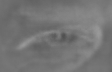
\includegraphics[width=4cm]{image/saturation.png}
 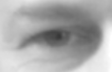
\includegraphics[width=4cm]{image/value.png}
 \caption{Décomposition du modèle HSV}
\end{figure}

Nous pouvons voir que la saturation est initulisable tel quel, car les valeurs sont beaucoup trop basse et trop proche.

% %TODO explication hsv Gaetan
% 
% \begin{figure}[H]
%  \center
%  
\includegraphics[width=4cm]{image/hue.png}
%  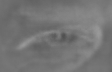
\includegraphics[width=4cm]{image/saturation.png}
%  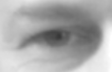
\includegraphics[width=4cm]{image/value.png}
%  \caption{Décomposition du modèle HSV}
% \end{figure}
% 
% solution -> calcul d'un masque pour réduire l'image pris en compte par canny
% étape de construction du masque : 
% \begin{itemize}
%  \item égalisation des trois composante de l'image de départ
%  \item passage de l'image en hsv
%  \item égalisation de la composante saturation%value
%  \item érosion de l'image
% \end{itemize}
% 
% %test avec le value mais a mon avis c pas tres stable -> voir masqueAv.png et masqueAp.png
% \begin{figure}[H]
%  \center
%  
\includegraphics[width=4cm]{image/resultatMasque.png}
%  \caption{Résultat du masque après application du masque}
% \end{figure}
% 
% saturation -> probleme sur la couleur de peau.
% 
% \begin{figure}[H]
%  \center
%  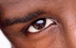
\includegraphics[width=4cm]{image/original_black.png}
%  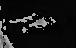
\includegraphics[width=4cm]{image/hue_black.png}
%  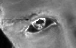
\includegraphics[width=4cm]{image/saturation_black.png}
%  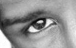
\includegraphics[width=4cm]{image/value_black.png}
%  \caption{Décomposition du modèle HSV avec une couleur de peau plus foncée}
% \end{figure}

\subsubsection{Le modèle YCbCr}

Nous avons testé un second modèle colorimètrique suite à l'étude des travaux de Evangelos Skodras et Nikolaos Fakotakis\cite{Skodras_2012ieee}.
En effet, leur étude montre que les différentes couleurs de peau de l'Homme ont à peu près la même valeur dans les deux
composantes du modèle YCbCr.\\

On peut voir sur le résultat de la décomposition de l'image que le canal représentant la première chominance met 
en évidence la pupille de l'oeil.
\begin{figure}[H]
 \center
 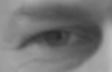
\includegraphics[width=4cm]{image/luminance.png}
 
\includegraphics[width=4cm]{image/chrominance1.png}
 
\includegraphics[width=4cm]{image/chrominance2.png}
 \caption{Décomposition du modèle YCbCr}
\end{figure}

\begin{figure}[H]
 \center
 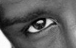
\includegraphics[width=4cm]{image/luminance_black.png}
 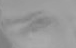
\includegraphics[width=4cm]{image/chrominance1_black.png}
 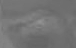
\includegraphics[width=4cm]{image/chrominance2_black.png}
 \caption{Décomposition du modèle YCbCr avec une couleur de peau plus foncée}
\end{figure}

Pour obtenir la valeur des différentes composantes de cet espace colorimètrique à partir
d'une image RGB il faut effectuer les calculs suivant :
$$Y = 0.299R + 0.587 G + 0.114 B$$
$$Cb = -0.1687R - 0.3313 G + 0.5B + 128$$
$$Cr = 0.5R -0.4187G -0.0813B + 128$$

\begin{figure}[H]
 \begin{tabular}{|c|c|c|c|c|c|c|}
  \hline
  couleur de peau & rouge & verte & bleu & luminance(Y) & chrominance 1(Cb) & chrominance 2(Cr)\\
  \hline
  blanc & 234 & 171 & 130 & 185 & 97 & 163 \\
  \hline
  bronzé & 175 & 112 & 95 & 129 & 109 & 161 \\
  \hline
  asiatique & 202 & 143 & 111 & 157 & 102 & 160\\
  \hline
 \end{tabular}
 \caption{Tableau des valeurs des couleurs de peau dans les espaces RGB et YCbCr}
\end{figure}

Nous pouvons voir avec ce tableau que la valeurs des deux chrominances sont très proche quelque soit
la couleur de la peau. Pour la suite des traitements, nous décidons de garder la chrominance 1 qui semble
varier un peu moins avec le changement de luminosité. En prenant le canal de la première chrominance et en 
trouvant le bon seuil pour la binarisation, nous obtenons une image comportant la forme de l'oeil au bon endroit.
Nous pouvons alors calculer le barycentre de la forme obtenu afin de récupérer le centre de l'oeil.

\begin{figure}[H]
 \center
 
\includegraphics[width=4cm]{image/result_yuv.png}
 \caption{Résulat après traitement sur la chominance 1}
\end{figure}

\subsection{Détection des contours avec des blobs}
Maintenant que nous obtenons une image binarisé comportant la forme de l'oeil, nous pouvons déterminer ou est
positionné le centre de l'oeil. Pour cela nous avons choisi l'utilisation de blob afin de résoudre un second 
problème que nous avons rencontré. Lorsque nous effectuons les traitements précédent sur la vidéo, nous avons
parfois des éléments qui perturbe la détection de contour comme des montures de lunette ou les cheveux de la personne 
filmé. Ces éléments peuvent faire partie des formes que nous récupérons lors de la binarisation. Les blobs
sont des objets qui vont détecter des formes dans une image, mais il est possible d'ajouter des caractèristiques
à ces blobs afin de récupérer seulement les formes qui possède ces caractèristiques.\\

Les blobs sont des éléments formé à partir d'une courbe 3D des fréquences d'une image.
%TODO en attente de la réinstallation scilab pour afficher des images pour les explication

Pour obtenir les blobs correspondant au yeux nous avons utilisé les paramètres :
\begin{itemize}
 \item la convexité : les yeux étant censé être une forme ovale, il ne devrait pas y'avoir de segment, entre 
 deux points, qui dépasse de la forme.
 \item l'aire de la forme : ce qui permet de ne pas prendre en compte les formes plus petites.
 \item la circularité de la forme : ce qui permet de ne pas prendre en compte les formes longue comme les cheveux
 sur le côté du visage.
\end{itemize}


\subsection{L'algorithme de Gabor}